\section{Tachometer på bil}

Tachometeret består af en TLE4905 \cite{lib:tle4905}
hallswitch, som fungerer ved at detektere magneter rettet i en bestemt retning. Kredsløbet er konstrueret således at hallswitchen trækker signalet til GND, når der detekteres en magnet. Kredsløbet bruger en meget lille strøm, målt til ca. 1.32mA, under tilstedeværelse af en magnet, uden er der målt en strøm på 5 $520\mu A$ . Med en forsyningsspænding på 5V bliver det til en effekt på 6.6mW, hvilket ikke betragtes som nogen EMC-mæssig trussel. Dog er der strømloops i systemet, som på tidspunkter vil være udsat for højfrekvente skift i strøm, hvilket er forsøgt forhindret ved at designe omtalte loops så små som muligt. Grundet det færdige prints størrelse, er det ikke muligt at placere det så tæt som muligt på hjulet som ønsket, hvorfor ledningerne ud til hall-switchen vil være snoede, således der fremkommer en common-mode støj.

\begin{figure}[h]
\centering
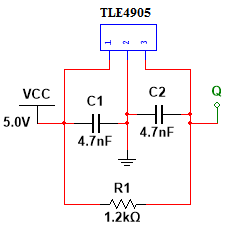
\includegraphics[scale=1]{../fig/billeder/tachometer_multisim.png}
\caption{Design af bilens tachometer i multisim.}
\label{fig:tachometer_multisim}
\end{figure}

Tachometeret er for så vidt ikke være truet af støjoverkobling fra andre kredsløb i systemet, da outputtet ligger fra 0V-5V, og der tælles på logisk LOW, ved Raspberry PI's GPIO. Dvs. at selvom der ligger 1V støj på outputtet, vil det ikke have nogen betydning for tachometerets præcision. Eftersom strømmene i kredsløbet er så små, vil der aldrig kunne induceres en spænding der er tilsvarene, hvilket betyder at der kan ses helt bort fra støjgenerering fra kredsløbet.  Dog er der for god ordens skyld sørget for, at placere kredsløbet så langt fra motorkredsløbet som fysik muligt. 

\clearpage